\documentclass{article}
\usepackage[margin=1in]{geometry}
\usepackage[utf8]{inputenc}
\usepackage{enumerate}
\usepackage{amsmath} 
\usepackage{natbib}
\usepackage{graphicx}
\usepackage{textcomp}
\usepackage{amsmath,amsfonts,amssymb, hyperref}

\title{Stanford CS 224n Assignment 5}
\author{Hanchung Lee}
\date{February 20, 2020}
\begin{document}

\maketitle
\section{Character-based convolutional encoder for NMT (36 points)}
\bigbreak
(a) (1 point) (written) In  Assignment 4 we used 256-dimensional word embeddings ($e_{word} =  256$), while in this assignment, it turns out that a character embedding size of 50 suffices ($e_{char} = 50$). In 1-2 sentences, explain one reason why the embedding size used for character-level embeddings is typically lower than that used for word embeddings.

\bigbreak
\noindent
\textbf{Answer:} There are only several dozens of alpha-numerical characters in writing but tens of thousands of words. Therefore character-level embeddings will have a much less dimension than word-level embeddings. More, because English is a phonetic language, the individual characters have much less if any meaning but individual words contains meanings, and the character dependencies are not as long ranged compare to words.

\bigbreak
\noindent
(b) (1 point) (written) Write down the total number of parameters in the character-based embedding model (Figure 2), then do the same for the word-based lookup embedding model (Figure 1).  Write each answer as a single expression (though you may show working) in terms of $e_{char}$, $k$, $e_{word}$, $V_{word}$ (the size of the word-vocabulary in the lookup embedding model) and $V_{char}$ (the size of the character-vocabulary in the character-based embedding model). Given that in our code, $k = 5$, $V_{word} \approx 50,000$ and $V_{char} = 96$, state which model has more parameters, and by what factor (e.g. twice as many? a thousand times as many?).

\bigbreak
\noindent
\textbf{Answer:} Char-based embedding total param is sum of the character indices embedding lookup, 1D convolution, and highway networks ($X_{proj}$ and $X_{gate}$).

\begin{align*}
\begin{split}
Param_{char-embeddings} &= Param_{emb} + Param_{conv} + Param_{highway} \\
&=(V_{char} \times e_{char}) + (e_{char} \times k \times e_{word} + e_{word}) + 2 \times(e_{word} \times e_{word} + e_{word})\\
&=(96 \times 50) + (50 \times 5 \times 256 + 256) + 2 \times(256 \times 256 + 256)\\
&=200,640
\end{split}\\
\begin{split}
Param_{word-embeddings} &= V_{word} \times e_{word}\\
&=50,000 \times 256\\
&=12,800,000
\end{split}
\end{align*}

\noindent 
Therefore, the word embedding model contains almost 64x as many parameters than character embedding model.

\bigbreak
\noindent
(c) (2 points) (written) In step 3 of the character-based embedding model, instead of using a 1D convnet, we could have used a RNN instead (e.g. feed the sequence of characters into a bi-directional LSTM and combine the hidden states using max-pooling). Explain one advantage of using a convolutional architecture rather than a recurrent architecture for this purpose, making it clear how the two contrast. Below is an example answer; you should give a similar level of detail and choose a different advantage.

\bigbreak
\noindent
\textbf{Answer:}
\begin{enumerate}[i)]
\item When a 1D convnet computes features for a given window of the input, those features depend on the window only – not any other inputs to the left or right. By contrast, a RNN needs to compute the hidden states sequentially, from left to right (and also right to left, if the RNN is bidirectional). Therefore, unlike a RNN, a convnet’s features can be computed in parallel, which means that convnets are generally faster, especially for long sequences.
\item 1D convnet uses a fixed window that extracts positional information on both sides all at the same time opposed to RNN have to unroll the time steps either uni-directionally or bi-directionally. This means it will have a faster training time. In addition, it can be designed to 'zoom' into a deeper latent features using more filters.
\item In this assignment, a 1D convnet has a $50 \times 5 \times 256 + 256 = 64,256$ parameters. An RNN with the same output dimension would have $(256\times256 + 256) = 65,792$ parameters trained over $k$ time steps. However, if we use alternate RNN models such as LSTM or GRU, the number of parameters will increase by 4x for LSTM and 3x for GRU.
\end{enumerate}

\bigbreak
\noindent
(d) (4 points) (written) In lectures we learned about both max-pooling and average-pooling. or each pooling method, please explain one advantage in  comparison to the other pooling method.  For each advantage, make it clear how the two contrast, and write to a similar level of detail as in the example given in the previous question

\bigbreak
\noindent
\textbf{Answer:}
\begin{center}
    \begin{tabular}{ |l|l|l| } 
        \hline
        & \textbf{Advantages} & \textbf{Disadvantages} \\ 
        \hline
        max pooling & Keeps only the strongest features while & Information loss from disregarding \\
        & zeroing out the lesser features & lessor features \\
        \hline
        average pooling & Maintains all of the features &  Stronger features got diluted by \\
         & & lesser smaller features\\
        \hline
    \end{tabular}
\end{center}

\bigbreak
\bigbreak
\noindent
(f) (4 points) (coding and written)  In the empty file \verb|highway.py|, implement the highway network as a \verb|nn.Module| class called \verb|Highway|. Once you’ve finished testing your module, write a short description of the tests you carried out,and why you believe they are sufficient.  The 4 points for this question are awarded based on your written description of the tests only.

\bigbreak
\noindent
\textbf{Answer:} Setup two test cases. Cannot be sure if the edge cases are tested or if the test cases are sufficient.
\begin{enumerate}[1]
\item Test initialization, shape of model weights, and if biases are implemented.
\item Test numerical results by first manually calculating the expected result using Numpy. Then feed the same Numpy input matrix to the \verb|nn.Module Highway| class. And finally compare the calculated Numpy output vs the output from \verb|Highway| module.
\end{enumerate}


\bigbreak
\bigbreak
\noindent
(g) (4 points)  (coding and written) In the empty file \verb|cnn.py|, implement the convolutional network as a \verb|nn.Module| class called \verb|CNN|. As in (f),  write code to thoroughly test your implementation.  Once you’ve finished testing your module, write a short description of the tests you carried out, and why you believe they are sufficient.As in (f), the 4 points are for your written description only.

\bigbreak
\noindent
\textbf{Answer:} Setup one test case1. Choose not to do manual hand calculation of 1D Conv as that might induce unintentional bugs. Doesn't make sense to write test cases to generate test case data.  Cannot be sure if the edge cases are tested or if the test cases are sufficient. EDIT: No, this is definitely not enough. At training small data set time, even when dimensions were fine, the kernel size being too big will throw off \verb|maxpool1d|. And Using \verb|ceil_mode=True| to fix that problem might cause the \verb|maxpool1d| dimension to be greater than 1. Perhaps need to write multiple test cases to test different types of inputs.
\begin{enumerate}
\item Test initialization, shape of model weights, and if biases are implemented.
\end{enumerate}

\section{Character-based LSTM decoder for NMT (26 points)}
\bigbreak
(e) (6 point) (coding) Report your test set BLEU score in your assignment write-up.  Also ensure that the output fileo \verb|outputs/test_outputs.txt| is present and unmodified – this will be included in your submission, and we’ll use it to verify your self-reported BLEU score. 

\bigbreak
\noindent
\textbf{Answer:} We ran the model using $batch-size=64$ vs default 32 and $max-epoch=60$ on RTX 2080 Ti on a local machine. It hit maximum number of epochs at around 34 hour mark. \verb|BLEU score| is \textbf{27.96}. Since the training loss and validation perplexity are still decreasing, however slow it might be, we suspect that we might achieve \verb|BLEU > 36| for the full 6 points. With a \verb|BLEU| score of 28, no points will be awarded. We will circle back in a later date to retrain the model. :(

\section{Analyzing NMT Systems (8 points)}
\bigbreak
(a) (2 points) (written) The following table shows some of the forms of the Spanish word \emph{traducir}, which means \emph{to translate}.
\begin{center}
    \begin{tabular}{ l l l } 
        \hline
        \textbf{Infinitive} & \textbf{traducir} & \textbf{to translate} \\ 
        \hline
        Present & traduzco & I translate \\
        & traduces & you translate \\
        & traduce & that you translate \\
        \hline
        Subjective & traduzca & that I translate \\
         & traduzcas& that you translate\\
        \hline
    \end{tabular}
\end{center}
Use \verb|vocab.json| to find (e.g. using \verb|grep|) which of these six forms are in the word-vocabulary, which consists of the 50,000 most frequent words in the training data for English and for Spanish. Superstrings don’t count (e.g.  having \verb|traducen| in the vocabulary is not a hit for \verb|traduce|).  State which of these six forms occur, and which do not.  Explain in one sentence why this is a bad thing forword-based NMT from Spanish to English.  Then explain in detail (approximately two sentences) how our new character-aware NMT model may overcome this problem.

\smallbreak
\noindent
\textbf{Answer:} \verb|traducir, idx:4630|, \verb|traduce, idx:7931|, and \verb|traduzco, idx:40991| are in the word-vocabulary while \verb|traducuces|, \verb|traduzca|, and \verb|traduzcas| are not in the vocabulary. This is a problem as the variations of the word will be out-of-vocabulary, get tagged as unknown, and not get recognized by the network. With a character-aware NMT, when an unknown word was encountered it will generate the OOV word use the character level decoder path and try to generate a character sequence using greedy search in the algorithm.

\bigbreak
\noindent
(b) i. (0.5 points) (written) In Assignments 1 and 2, we investigated word embeddings created via algorithms such a Word2Vec, and found that for these embeddings, semantically similar words are close together in the embedding space. In this exercise, we’ll compare this with the word embeddings constructed using the CharCNN trained in our NMT system. For each word, report the single closest neighbor.  For your convenience, for each example takea screenshot of all the nearest words (so you can compare with the CharCNN embeddings).
\bigbreak
\noindent
\textbf{Answer:} As follows. Screenshot included in ii.
\begin{itemize}
    \item \verb|financial| \textrightarrow{} economic
    \item \verb|neuron| \textrightarrow{} neurons
    \item \verb|Francisco| \textrightarrow{} san
    \item \verb|naturally| \textrightarrow{} occuring
    \item \verb|expectation| \textrightarrow{} operator
\end{itemize}

\bigbreak
\noindent
ii. (0.5 points)  (written) The TensorFlow embedding projector also allows you to upload your own data – you may find this useful in your projects! Download  the  character-based  word  embeddings  obtained  from  our  implementation  of  the character-aware NMT model from this link. Navigate to https://projector.tensorflow.org/, select \verb|Load Data|, and upload the files \verb|character-embeddings.txt| (the embeddings themselves) and \verb|metadata.txt| (the words associated with the embeddings). 
Now look at the nearest neighbors of the same words.  Again, report the single closest neighbors with dataset \verb|Word2Vec All| and take screenshots for yourself.

\bigbreak
\noindent
\textbf{Answer:} Please see attached images below.
\begin{figure}
    \centering
    \subfloat{{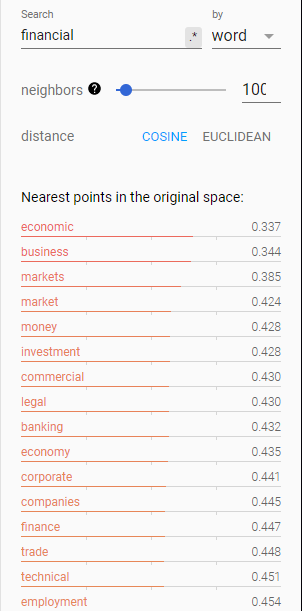
\includegraphics[width=5cm]{q3b_tf1.png}}}
    \qquad
    \subfloat{{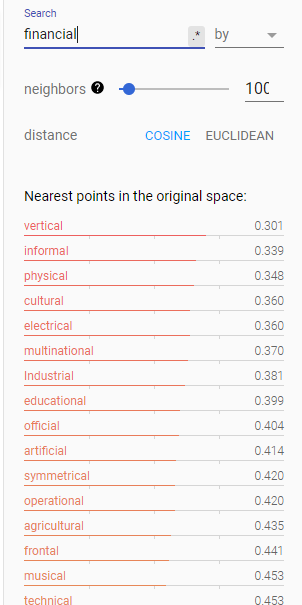
\includegraphics[width=5cm]{q3b_custom1.png}}}
    \caption{financial. Word2Vec Left, CharCNN Right}
    \label{fig:example}
\end{figure}
\begin{figure}
    \centering
    \subfloat{{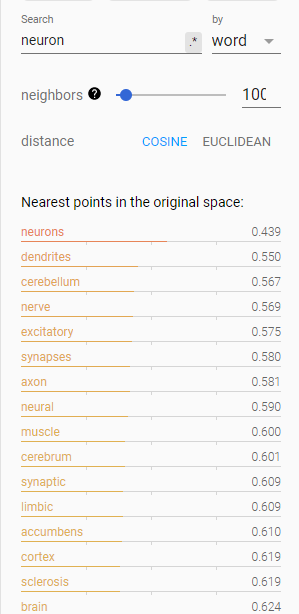
\includegraphics[width=5cm]{q3b_tf2.png}}}
    \qquad
    \subfloat{{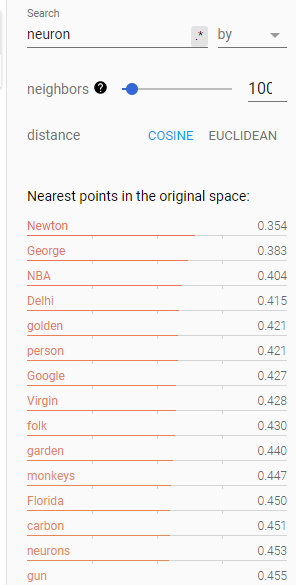
\includegraphics[width=5cm]{q3b_custom2.png}}}
    \caption{neuron. Word2Vec Left, CharCNN Right}
    \label{fig:example}
\end{figure}
\begin{figure}
    \centering
    \subfloat{{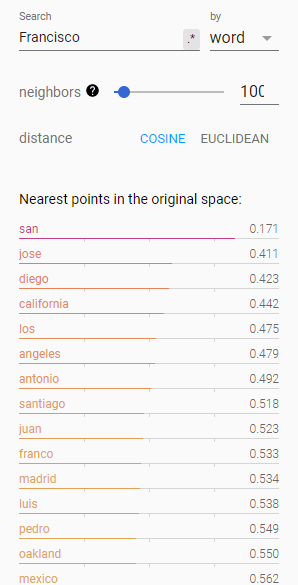
\includegraphics[width=5cm]{q3b_tf3.png}}}
    \qquad
    \subfloat{{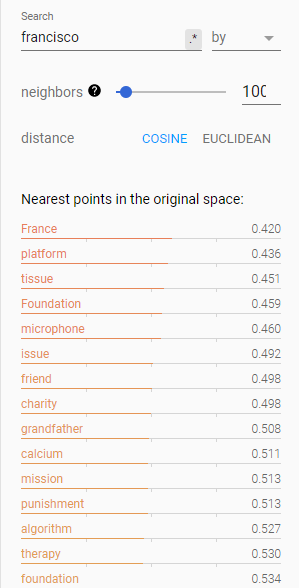
\includegraphics[width=5cm]{q3b_custom3.png}}}
    \caption{Francisco. Word2Vec Left, CharCNN Right}
    \label{fig:example}
\end{figure}
\begin{figure}
    \centering
    \subfloat{{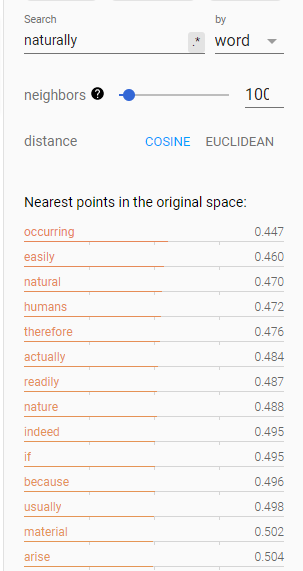
\includegraphics[width=5cm]{q3b_tf4.png}}}
    \qquad
    \subfloat{{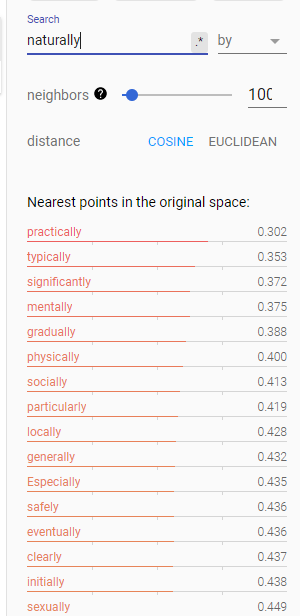
\includegraphics[width=5cm]{q3b_custom4.png}}}
    \caption{naturally. Word2Vec Left, CharCNN Right}
    \label{fig:example}
\end{figure}
\begin{figure}
    \centering
    \subfloat{{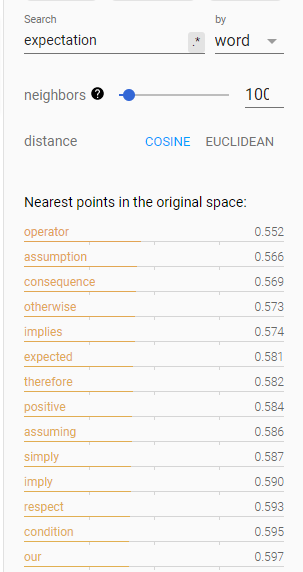
\includegraphics[width=5cm]{q3b_tf5.png}}}
    \qquad
    \subfloat{{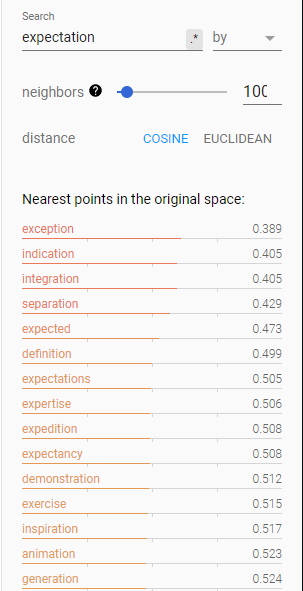
\includegraphics[width=5cm]{q3b_custom5.png}}}
    \caption{expectation. Word2Vec Left, CharCNN Right}
    \label{fig:example}
\end{figure}

\clearpage
\bigbreak
\noindent
iii. (3 points)  (written) Compare the closest neighbors found by the two methods:  briefly describe what kind of similarity is modeled by Word2Vec,  and what kind of similarity is modeled by the CharCNN. Explain in detail (2-3 sentences) how the differences in the methodology of Word2Vec and a CharCNN explain the differences you have found.
   
\bigbreak
\noindent
\textbf{Answer:} Word2Vec models focuses on sematic similarity between neighboring words, i.e., word vectors is about its context. CharCNN model looks at the structural similarity of our particular dataset using a window-based feature, so words similar in word structure will be closer in feature space.


\bigbreak
\noindent
(c) (2 points) (written) As in Assignment 4, we’ll take a look at the outputs of the model that you have trained! The test set translations your model generated in 2(e) should be located in the outputs directory at: \verb|outputs/test_outputs.txt|. We also provided translations from a word-based model from our Assignment 4 model in the file \verb|outputs/test_outputs_a4.txt|.
\smallbreak
\noindent
Find places where the word-based model produced \verb|<UNK>|, and compare to what the character-based decoder did. Find one example where the character-based decoder produced an acceptable translation in place of \verb|<UNK>|, and one example where the character-based decoder produced an incorrect translation in place of \verb|<UNK>|. As in Assignment 4, ‘acceptable’ and ‘incorrect’ doesn’t just  mean  ‘matches  or  doesn’t  match  the  reference  translation’ – use your own judgment (and Google Translate, if necessary).

\bigbreak
\noindent
\textbf{Answer:} Using our BLEU score 24.35 model, here are the differences.
\begin{center}
    \begin{tabular}{ l l l } 
        \hline
        & \textbf{Reference Translation} & \textbf{CharCNN Translation} \\ 
        \hline
        Acceptable & Well, the next day we were in Cleveland & Well, the next day we in Cleveland. \\
         & I was in awe. & I was astounded . \\
        \hline
        Incorrect & We took a look at her, we laughed, we cried, & We went to see it, we laughed, we, and \\
        & and we knew that she needed to be in a hospice. & we realized that she needed to be customized. \\
        \hline
    \end{tabular}
\end{center}

\end{document}